\section{Bloch states and band structure}\label{sec:3.2}

An electron in silicon moves in a potential that repeats itself after every lattice vector: the attraction of the clamped nuclei, the repulsion of the other electrons, and the exchange and correlation effects that come with them (\cref{sec:2.3}). The full problem is a many-electron one. Most of what a dark-matter rate needs, however, can be understood with each electron moving independently in an effective potential $U(\vect{r})$ with the periodicity of the lattice, $U(\vect{r} + \vect{R}) = U(\vect{r})$. Density-functional theory supplies the best such potential and tells us what it leaves out (\cref{sec:3.4}). Here $U$ is any lattice-periodic function, and its periodicity alone fixes the form of the states and the momentum transfers that connect them. Bands and gaps are understood in two opposite limits, nearly free electrons and tight binding. We then compute the two matrix elements that every electronic rate in this book contains: that of $\ee^{\ii\vect{q}\cdot\vect{r}}$, to which dark matter couples, and that of the velocity, to which light couples. We follow Refs.~\cite[Chaps.~8--10]{ashcroft1976solid}, \cite[Chap.~3]{harrison1980electronic} and \cite[Chap.~2]{yu2010fundamentals}.

\subsection{Bloch's theorem}

The one-electron Hamiltonian is
\begin{equation}
  H_{\mathrm{e}} = \frac{\op{\vect{p}}^2}{2m_e} + U(\vect{r}), \qquad U(\vect{r} + \vect{R}) = U(\vect{r}) ,
  \label{eq:3.2-He}
\end{equation}
with $\op{\vect{p}} = -\ii\nabla$. We keep the electron spinless and count the two spin states with an explicit factor of 2; spin--orbit coupling, which mixes them, enters in \cref{sec:3.3}. The translation operator of \cref{sec:3.1}, acting now on one electron, is $(T_{\vect{R}}\psi)(\vect{r}) = \psi(\vect{r} + \vect{R})$. The kinetic energy is unchanged by any translation, and $U$ by a lattice translation, so every $T_{\vect{R}}$ commutes with $H_{\mathrm{e}}$. The argument that led to \cref{eq:3.1-crystalmomentum} then applies to a single electron: the eigenstates of $H_{\mathrm{e}}$ can be chosen so that $\psi(\vect{r} + \vect{R}) = \ee^{\ii\vect{k}\cdot\vect{R}}\psi(\vect{r})$ for every $\vect{R}$, with $\vect{k}$ in the first Brillouin zone and on the Born--von Karman grid of \cref{eq:3.1-kgrid}. Define $u(\vect{r}) = \ee^{-\ii\vect{k}\cdot\vect{r}}\psi(\vect{r})$. It is periodic, since $u(\vect{r} + \vect{R}) = \ee^{-\ii\vect{k}\cdot\vect{r}}\ee^{-\ii\vect{k}\cdot\vect{R}}\,\ee^{\ii\vect{k}\cdot\vect{R}}\psi(\vect{r}) = u(\vect{r})$. Each eigenstate is therefore a plane wave modulated by a function with the period of the lattice:
\begin{keyresult}[Bloch's theorem]
\begin{equation}
  \psi_{n\vect{k}}(\vect{r}) = \frac{1}{\sqrt N}\,\ee^{\ii\vect{k}\cdot\vect{r}}\,u_{n\vect{k}}(\vect{r}), \qquad
  u_{n\vect{k}}(\vect{r} + \vect{R}) = u_{n\vect{k}}(\vect{r}), \qquad
  \int_\Omega\dd^3r\,|u_{n\vect{k}}|^2 = 1 .
  \label{eq:3.2-bloch}
\end{equation}
Equivalently, $\psi_{n\vect{k}}(\vect{r} + \vect{R}) = \ee^{\ii\vect{k}\cdot\vect{R}}\psi_{n\vect{k}}(\vect{r})$. The state is normalized to one over the crystal of volume $\Vol = N\Omega$, and its periodic part to one over a cell.
\end{keyresult}
The two normalizations agree because $|\psi_{n\vect{k}}|^2 = |u_{n\vect{k}}|^2/N$ is periodic and the crystal holds $N$ cells; these are the conventions of \cref{app:A.5}. The label $n$, the \emph{band index}, appears because there are many solutions at each $\vect{k}$. Inserting $\psi = N^{-1/2}\ee^{\ii\vect{k}\cdot\vect{r}}u$ into $H_{\mathrm{e}}\psi = \varepsilon\psi$ and using $\op{\vect{p}}\,\ee^{\ii\vect{k}\cdot\vect{r}}u = \ee^{\ii\vect{k}\cdot\vect{r}}(\op{\vect{p}} + \vect{k})u$ leaves an equation for $u$ alone,
\begin{equation}
  H_{\vect{k}}\,u_{n\vect{k}} = \varepsilon_{n\vect{k}}\,u_{n\vect{k}}, \qquad
  H_{\vect{k}} \equiv \ee^{-\ii\vect{k}\cdot\vect{r}}H_{\mathrm{e}}\,\ee^{\ii\vect{k}\cdot\vect{r}} = \frac{(\op{\vect{p}} + \vect{k})^2}{2m_e} + U(\vect{r}) ,
  \label{eq:3.2-Hk}
\end{equation}
to be solved in one cell with periodic boundary conditions. Like a particle in a box, $H_{\vect{k}}$ has a discrete spectrum at each $\vect{k}$, which we order as $\varepsilon_{1\vect{k}} \le \varepsilon_{2\vect{k}} \le \dots$. Since $\vect{k}$ enters $H_{\vect{k}}$ as a parameter, each \emph{band energy} $\varepsilon_{n\vect{k}}$ varies continuously with $\vect{k}$ and sweeps out an energy band; the set of all of them, plotted along lines through the zone, is the \emph{band structure}. The bands are periodic in reciprocal space: $\ee^{-\ii\vect{G}\cdot\vect{r}}u_{n\vect{k}}$ is periodic and satisfies $H_{\vect{k}+\vect{G}}\,\ee^{-\ii\vect{G}\cdot\vect{r}}u_{n\vect{k}} = \ee^{-\ii\vect{G}\cdot\vect{r}}H_{\vect{k}}u_{n\vect{k}}$, so $\varepsilon_{n,\vect{k}+\vect{G}} = \varepsilon_{n\vect{k}}$. We use this freedom to identify the states themselves, $\psi_{n,\vect{k}+\vect{G}} = \psi_{n\vect{k}}$, which is the \emph{periodic gauge} of \cref{eq:A.5-periodic}. A crystal momentum outside the first zone can then be used directly.

A Bloch state is not a state of definite momentum. Its periodic part is a Fourier series over reciprocal-lattice vectors, and we write it in the convention of plane-wave codes (\cref{app:A.3}),
\begin{equation}
  u_{n\vect{k}}(\vect{r}) = \frac{1}{\sqrt\Omega}\sum_{\vect{G}}c_{n\vect{k}}(\vect{G})\,\ee^{\ii\vect{G}\cdot\vect{r}}, \qquad
  \psi_{n\vect{k}}(\vect{r}) = \frac{1}{\sqrt \Vol}\sum_{\vect{G}}c_{n\vect{k}}(\vect{G})\,\ee^{\ii(\vect{k}+\vect{G})\cdot\vect{r}}, \qquad
  \sum_{\vect{G}}|c_{n\vect{k}}(\vect{G})|^2 = 1 .
  \label{eq:3.2-pw}
\end{equation}
The coefficient $c_{n\vect{k}}(\vect{G})$ multiplies $\ee^{+\ii\vect{G}\cdot\vect{r}}$, so it is the lattice Fourier component of \cref{eq:A.3-periodic} at $-\vect{G}$, times $\Omega^{1/2}$. The electron in state $n\vect{k}$ has the momenta $\vect{k} + \vect{G}$, with probabilities $|c_{n\vect{k}}(\vect{G})|^2$. A smooth valence state is dominated by a few small $\vect{G}$; the part of the wavefunction near the nuclei, where it oscillates rapidly, puts weight at large $|\vect{G}|$, and it is this tail that a momentum transfer of many keV probes (\cref{sec:3.5}).

The same expansion turns \cref{eq:3.2-Hk} into an algebraic equation and provides a second proof of Bloch's theorem. Write the potential as $U(\vect{r}) = \sum_{\vect{G}''}U_{\vect{G}''}\,\ee^{-\ii\vect{G}''\cdot\vect{r}}$, with the components $U_{\vect{G}} = \Omega^{-1}\int_\Omega\dd^3r\,\ee^{\ii\vect{G}\cdot\vect{r}}U(\vect{r})$ of \cref{eq:A.3-periodic}. Acting on a plane wave, $U$ produces $U(\vect{r})\,\ee^{\ii(\vect{k}+\vect{G}')\cdot\vect{r}} = \sum_{\vect{G}''}U_{\vect{G}''}\,\ee^{\ii(\vect{k}+\vect{G}'-\vect{G}'')\cdot\vect{r}}$. Collecting the coefficient of $\ee^{\ii(\vect{k}+\vect{G})\cdot\vect{r}}$ in $H_{\mathrm{e}}\psi_{n\vect{k}} = \varepsilon_{n\vect{k}}\psi_{n\vect{k}}$ picks the term $\vect{G}'' = \vect{G}' - \vect{G}$, and
\begin{equation}
  \Bigl[\frac{(\vect{k} + \vect{G})^2}{2m_e} - \varepsilon_{n\vect{k}}\Bigr]c_{n\vect{k}}(\vect{G}) + \sum_{\vect{G}'}U_{\vect{G}'-\vect{G}}\,c_{n\vect{k}}(\vect{G}') = 0 .
  \label{eq:3.2-central}
\end{equation}
A periodic potential couples a plane wave only to those that differ from it by a reciprocal-lattice vector. A state built from one $\vect{k}$ and its translates $\vect{k} + \vect{G}$ stays among them, which is Bloch's theorem again. The matrix $(\vect{k}+\vect{G})^2\delta_{\vect{G}\vect{G}'}/2m_e + U_{\vect{G}'-\vect{G}}$ is Hermitian, since a real $U$ has $U_{-\vect{G}} = U^*_{\vect{G}}$. Its eigenvalues are the $\varepsilon_{n\vect{k}}$, and its eigenvectors the $c_{n\vect{k}}(\vect{G})$. A plane-wave code diagonalizes this matrix, truncated at a cutoff in $|\vect{k}+\vect{G}|$ (\cref{sec:3.5}).

Bloch states with different $\vect{k}$ are orthogonal, because they belong to different eigenvalues of the unitary $T_{\vect{R}}$, and states with the same $\vect{k}$ and different $n$ are orthogonal as eigenvectors of the Hermitian $H_{\vect{k}}$. Together they form an orthonormal basis, and the change of basis of \cref{eq:2.3-basis} turns the plane-wave operators of \cref{sec:2.3} into operators $c^\dagger_{n\vect{k}s}$ and $c_{n\vect{k}s}$ that create and destroy an electron of spin $s$ in a Bloch state. For independent electrons the Hamiltonian is $\sum_{n\vect{k}s}\varepsilon_{n\vect{k}}\,c^\dagger_{n\vect{k}s}c_{n\vect{k}s}$, and in thermal equilibrium the \emph{occupation} of a state is, by \cref{eq:2.5-nF},
\begin{equation}
  f_{n\vect{k}} = \langle c^\dagger_{n\vect{k}s}c_{n\vect{k}s}\rangle = n_{\mathrm{F}}(\varepsilon_{n\vect{k}} - \mu_{\mathrm{ch}}) .
  \label{eq:3.2-fnk}
\end{equation}
Each band holds $2N$ electrons, as \cref{sec:3.1} counted. In silicon the eight valence electrons per cell fill the four lowest bands, and a gap of about an electronvolt separates them from the next ones (\cref{sec:3.3}). At any temperature at which a detector runs, $f_{n\vect{k}} = 1$ in these four bands and $0$ above them, to an accuracy set by $\ee^{-\Eg/2T}$, the factor that the intrinsic carrier density of \cref{eq:3.3-ni} carries. Two questions follow: where such gaps come from, and how $\ee^{\ii\vect{q}\cdot\vect{r}}$ connects the states on either side of them.

\subsection{Nearly free electrons}

Switch the potential off. The eigenstates of \cref{eq:3.2-central} are then single plane waves, $c_{n\vect{k}}(\vect{G}) = \delta_{\vect{G},\vect{G}_n}$ for some vector $\vect{G}_n$ that labels the band, with energies $\varepsilon^0_{\vect{k}+\vect{G}_n}$. Here $\varepsilon^0_{\vect{k}} = k^2/2m_e$ is the free-electron energy at wavevector $\vect{k}$, inside the zone or not. Nothing physical has changed: the free parabola has been cut into pieces and each piece shifted by a reciprocal-lattice vector into the first zone, so that at a given $\vect{k}$ the bands are the parabolas centered on all the $-\vect{G}$. This is the \emph{empty-lattice} band structure, drawn dashed in \cref{fig:3-nfe}(a). Its bands cross wherever two plane waves have equal energy, $\varepsilon^0_{\vect{k}} = \varepsilon^0_{\vect{k}-\vect{G}}$, that is, on the planes $\vect{k}\cdot\vect{G} = |\vect{G}|^2/2$ that bisect the reciprocal-lattice vectors. These are the Bragg planes whose pieces bound the Brillouin zone (\cref{sec:3.1}).

Now let $U$ be weak. Away from a crossing, the coupling $U_{\vect{G}'-\vect{G}}$ mixes plane waves whose energies differ by much more than $|U|$, and second-order perturbation theory shifts each level by $\sum_{\vect{G}\neq0}|U_{\vect{G}}|^2/(\varepsilon^0_{\vect{k}} - \varepsilon^0_{\vect{k}-\vect{G}})$, a small correction. Near a crossing, however, two plane waves are degenerate and perturbation theory in this form fails. We keep just those two, $\ee^{\ii\vect{k}\cdot\vect{r}}$ and $\ee^{\ii(\vect{k}-\vect{G})\cdot\vect{r}}$. \Cref{eq:3.2-central} for the coefficients $c(0)$ and $c(-\vect{G})$ reads
\begin{equation}
  \begin{pmatrix} \varepsilon^0_{\vect{k}} & U_{-\vect{G}} \\ U_{\vect{G}} & \varepsilon^0_{\vect{k}-\vect{G}} \end{pmatrix}
  \begin{pmatrix} c(0) \\ c(-\vect{G}) \end{pmatrix} = \varepsilon \begin{pmatrix} c(0) \\ c(-\vect{G}) \end{pmatrix},
  \label{eq:3.2-twowave}
\end{equation}
where the diagonal $U_0$, a constant shift, has been absorbed into the energy zero. The eigenvalues are
\begin{equation}
  \varepsilon_\pm = \frac{\varepsilon^0_{\vect{k}} + \varepsilon^0_{\vect{k}-\vect{G}}}{2} \pm \sqrt{\Bigl(\frac{\varepsilon^0_{\vect{k}} - \varepsilon^0_{\vect{k}-\vect{G}}}{2}\Bigr)^2 + |U_{\vect{G}}|^2} .
  \label{eq:3.2-epm}
\end{equation}
Far from the plane the square root tends to $|\varepsilon^0_{\vect{k}} - \varepsilon^0_{\vect{k}-\vect{G}}|/2$, and the two free parabolas are recovered. On the plane the two free energies are equal, and the levels are pushed apart symmetrically:
\begin{keyresult}[Nearly-free-electron gap]
On the Bragg plane $\vect{k}\cdot\vect{G} = |\vect{G}|^2/2$, a weak periodic potential splits the two degenerate plane waves into $\varepsilon_\pm = \varepsilon^0_{\vect{k}} \pm |U_{\vect{G}}|$. The gap,
\begin{equation}
  \varepsilon_+ - \varepsilon_- = 2|U_{\vect{G}}| ,
  \label{eq:3.2-gap}
\end{equation}
is set by the Fourier component of the potential at the reciprocal-lattice vector that the plane bisects. It holds to first order in $U$, as long as $|U_{\vect{G}}|$ is small compared with the energy separation to the next plane waves.
\end{keyresult}
At the zone boundary the band structure therefore has a gap, and no state of the crystal has an energy inside it, whatever the direction of $\vect{k}$ along the plane. Whether the gaps on different faces of the zone overlap in energy and leave a gap for the whole crystal depends on the sizes of the $U_{\vect{G}}$ and on the shape of the zone. In a nearly-free metal such as aluminium they do not, and a Fermi surface survives~\cite[Chap.~9]{ashcroft1976solid}. Note that a component that vanishes by extinction (\cref{we:3-diamond}) opens no gap at first order. In silicon, the square faces of the zone bisect $\vect{G}_{200}$, and $U_{\vect{G}_{200}} = 0$ exactly, by the glide symmetry of the diamond structure (\cref{we:3-diamond}, \cref{app:C.17}).

The states at the gap are standing waves. For a potential with inversion symmetry and real $U_{\vect{G}} = U_{-\vect{G}}$, the eigenvectors of \cref{eq:3.2-twowave} on the plane are $c(-\vect{G}) = \pm c(0)$, so that $\psi \propto \ee^{\ii\vect{G}\cdot\vect{r}/2} \pm \ee^{-\ii\vect{G}\cdot\vect{r}/2}$ for $\vect{k} = \vect{G}/2$: a cosine and a sine of $\vect{G}\cdot\vect{r}/2$. The two have the same kinetic energy, but the cosine piles the electron density up at the points where $\vect{G}\cdot\vect{r}$ is a multiple of $2\pi$, the lattice planes, and the sine piles it up halfway between them. If the potential is attractive at the planes, $U_{\vect{G}} < 0$, the cosine lies lower by $|U_{\vect{G}}|$ and the sine higher by the same amount. A running wave at the boundary would be Bragg-reflected into its partner at $\vect{k} - \vect{G}$; the two standing waves are what remains, and both carry no current. The group velocity, the slope of the band (\cref{eq:3.2-vg} below), vanishes on the Bragg plane in the direction of $\vect{G}$, and the bands meet the zone boundary with zero slope, as \cref{fig:3-nfe}(a) shows.

\begin{figure}[tbp]
  \centering
  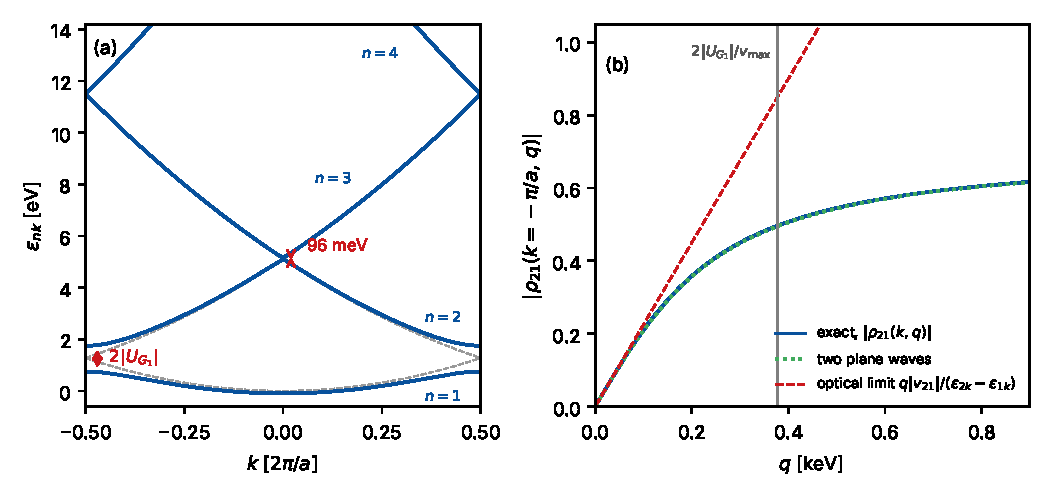
\includegraphics[width=\linewidth]{figures/ch03/fig3_4.pdf}
  \caption{Nearly free electrons in one dimension, for the potential $U(x) = 2U_{G_1}\cos(G_1x)$ with $G_1 = 2\pi/a$, $a = \SI{5.431}{\angstrom}$ (the lattice constant of silicon, used only to set the scale) and $U_{G_1} = \SI{-0.5}{eV}$. The bands are computed by diagonalizing \cref{eq:3.2-central} in 25 plane waves $\ee^{\ii(k+jG_1)x}$, $|j| \le 12$. (a)~The four lowest bands $\varepsilon_{nk}$ (solid) and the free-electron parabolas $(k + jG_1)^2/2m_e$ folded into the first zone (dashed). The first gap, at the zone boundary $k = \pm\pi/a$, is \SI{0.998}{eV}, close to $2|U_{G_1}| = \SI{1}{eV}$; the second, at $k = 0$, is \SI{96}{meV}, second order in $U_{G_1}$, since the potential has no component at $2G_1$. (b)~The density vertex $|\rho_{21}(k, q)|$ between the two lowest bands at $k = -\pi/a$, for momentum transfers $0 < q < \SI{0.9}{keV}$, which keep $k + q$ in the first zone. Solid: the full calculation. Dotted: the two-plane-wave model, indistinguishable at this scale. Dashed: the optical limit $q|v_{21}(k)|/(\varepsilon_{2k} - \varepsilon_{1k})$. The vertical line marks the smallest momentum transfer at which dark matter can deposit \SI{1}{eV}, $2|U_{G_1}|/v_{\mathrm{max}} = \SI{0.38}{keV}$ for $v_{\mathrm{max}} = 2.650\times10^{-3}$.}
  \label{fig:3-nfe}
\end{figure}

\begin{workedexample}{The one-dimensional gap}\label{we:3-gap1d}
Take the one-dimensional potential $U(x) = 2U_{G_1}\cos(G_1x)$, whose only components are $U_{\pm G_1} = U_{G_1}$, with $U_{G_1} = \SI{-0.5}{eV}$ and the period $a = \SI{5.431}{\angstrom}$, so that $G_1 = 2\pi/a = \SI{2283}{eV}$. The potential is attractive at the lattice sites, $U(0) = \SI{-1}{eV}$. The free-electron energy at the zone boundary, $k = G_1/2$, is
\begin{equation*}
  \varepsilon^0_{G_1/2} = \frac{(G_1/2)^2}{2m_e} = \frac{(\SI{1141.5}{eV})^2}{2\times\SI{511.0}{keV}} = \SI{1.275}{eV} ,
\end{equation*}
and \cref{eq:3.2-epm} puts the band edges at $\SI{1.275}{eV} \mp \SI{0.5}{eV}$, that is, at 0.775 and \SI{1.775}{eV}, with the gap $2|U_{G_1}| = \SI{1.000}{eV}$. The lower edge is the cosine, concentrated on the sites, and the upper edge the sine, concentrated between them; the full calculation of \cref{fig:3-nfe} confirms that $|\psi|^2$ of the lower state vanishes at $x = a/2$, and that of the upper state at $x = 0$.

Diagonalizing \cref{eq:3.2-central} in 25 plane waves gives the edges 0.752 and \SI{1.749}{eV}, and the gap \SI{0.998}{eV}. The lower edge has moved down by \SI{0.023}{eV} and the upper by \SI{0.026}{eV}. The shift comes from the next plane waves, $\ee^{\ii(G_1/2 + G_1)x}$ and $\ee^{\ii(-G_1/2 - G_1)x}$, which each of the two boundary states can reach with one factor of $U_{G_1}$. Their energy is $9\times\SI{1.275}{eV} = \SI{11.47}{eV}$, and second-order perturbation theory yields $U_{G_1}^2/(\SI{1.275}{eV} - \SI{11.47}{eV}) = \SI{-0.025}{eV}$ for each edge, the average of the two computed shifts. The gap $2|U_{G_1}|$ is thus accurate to \SI{0.2}{\percent}, although $|U_{G_1}|$ is \SI{40}{\percent} of the kinetic energy at the boundary.

The second gap is a different matter. It opens at $k = 0$, where the plane waves $\ee^{\pm\ii G_1x}$ are degenerate at $\varepsilon^0_{G_1} = \SI{5.099}{eV}$. They differ by $2G_1$, and $U_{2G_1} = 0$, so they are not coupled directly. They are coupled at second order through the plane wave $\ee^{\ii0x}$, with the effective matrix element $U_{G_1}^2/(\varepsilon^0_{G_1} - \varepsilon^0_0) = \SI{0.049}{eV}$, and the two-level splitting is twice this, \SI{0.098}{eV}. The full calculation finds \SI{0.096}{eV}. A gap at a Bragg plane is first order in the component of $U$ at that $\vect{G}$, and higher order if that component vanishes. This is what happens on the square faces of the silicon zone, where the extinction of $\vect{G}_{200}$ removes the first-order term.
\end{workedexample}

Silicon is not in the regime where these estimates are quantitative. A three-dimensional gap requires the gaps on all faces of the zone to overlap in energy, and in silicon the band edges lie at different crystal momenta (\cref{sec:3.3}). Its potential is not weak either: the free-electron energy at $\mathrm{L}$ is $|\vect{G}_{111}|^2/8m_e = \SI{3.82}{eV}$, and the strong attraction of the ion cores mixes many plane waves into each state, a problem that the pseudopotentials of \cref{sec:3.5} remove. What survives is the mechanism. Gaps open where the free-electron energy surfaces cross the Bragg planes, and they are set by the Fourier components of the potential. The opposite limit, in which electrons hop between atomic orbitals, explains why silicon has a gap where it does.

\subsection{Tight binding and the \texorpdfstring{$sp^3$}{sp3} bond}

A silicon atom in the gas has two $3s$ and two $3p$ electrons in sharp atomic levels. Bring the atoms together into a crystal of $N$ cells, and each atomic level of each atom in the cell broadens into a band of $N$ states, because the electrons can now hop from atom to atom. When the hopping is weak compared with the spacing of the atomic levels, the natural starting point is the atomic orbitals, not plane waves. This is the \emph{tight-binding} method, or the linear combination of atomic orbitals (LCAO).

Let $\varphi^{\mathrm{at}}_j(\vect{r})$ be atomic orbitals, with $j$ labeling both the orbital and the site $\vect{\tau}_\kappa$ of the basis on which it is centered, and $\varphi^{\mathrm{at}}_{j\vect{R}}(\vect{r}) = \varphi^{\mathrm{at}}_j(\vect{r} - \vect{R})$ its copy in cell $\vect{R}$. No single orbital has the form \cref{eq:3.2-bloch}, but the \emph{Bloch sum}
\begin{equation}
  |j\vect{k}\rangle = \frac{1}{\sqrt N}\sum_{\vect{R}}\ee^{\ii\vect{k}\cdot\vect{R}}\,|\varphi^{\mathrm{at}}_{j\vect{R}}\rangle ,
  \label{eq:3.2-blochsum}
\end{equation}
does: translating it by a lattice vector $\vect{R}'$ relabels the sum and multiplies it by $\ee^{\ii\vect{k}\cdot\vect{R}'}$. Since $H_{\mathrm{e}}$ commutes with lattice translations, it does not connect Bloch sums of different $\vect{k}$, and we look for the states as $|\psi_{n\vect{k}}\rangle = \sum_jC_{nj}(\vect{k})\,|j\vect{k}\rangle$, with one coefficient per orbital in the cell. The matrix elements between Bloch sums reduce to sums over one lattice vector. Translation invariance gives $\langle\varphi^{\mathrm{at}}_{j\vect{R}}|H_{\mathrm{e}}|\varphi^{\mathrm{at}}_{j'\vect{R}'}\rangle = \langle\varphi^{\mathrm{at}}_{j\vect{0}}|H_{\mathrm{e}}|\varphi^{\mathrm{at}}_{j',\vect{R}'-\vect{R}}\rangle$. The double sum over $\vect{R}$ and $\vect{R}'$ in $\langle j\vect{k}|H_{\mathrm{e}}|j'\vect{k}\rangle$ becomes $N$ times a single sum over $\vect{R}'' = \vect{R}' - \vect{R}$:
\begin{equation}
  H^{\mathrm{TB}}_{jj'}(\vect{k}) = \sum_{\vect{R}}\ee^{\ii\vect{k}\cdot\vect{R}}\,\langle\varphi^{\mathrm{at}}_{j\vect{0}}|H_{\mathrm{e}}|\varphi^{\mathrm{at}}_{j'\vect{R}}\rangle, \qquad
  S^{\mathrm{ov}}_{jj'}(\vect{k}) = \sum_{\vect{R}}\ee^{\ii\vect{k}\cdot\vect{R}}\,\langle\varphi^{\mathrm{at}}_{j\vect{0}}|\varphi^{\mathrm{at}}_{j'\vect{R}}\rangle .
  \label{eq:3.2-HS}
\end{equation}
Orbitals on neighboring atoms overlap, so the Bloch sums are not orthonormal, and the \emph{overlap matrix} $S^{\mathrm{ov}}(\vect{k})$ is not the identity. Requiring the energy $\langle\psi|H_{\mathrm{e}}|\psi\rangle/\langle\psi|\psi\rangle$ to be stationary with respect to the coefficients $C^*_{nj}$ turns the Schr\"odinger equation into the generalized eigenvalue problem
\begin{equation}
  \sum_{j'}H^{\mathrm{TB}}_{jj'}(\vect{k})\,C_{nj'}(\vect{k}) = \varepsilon_{n\vect{k}}\sum_{j'}S^{\mathrm{ov}}_{jj'}(\vect{k})\,C_{nj'}(\vect{k}) .
  \label{eq:3.2-LCAO}
\end{equation}
There are as many bands as orbitals in the cell. Of course, the result is only as good as the basis, which in practice is a few orbitals per atom; the payoff is that a handful of numbers, the on-site energies and the hopping and overlap integrals between neighbors, fix the band structure.

The simplest case is one $s$ orbital per site of a Bravais lattice, which yields one band, $n = 1$. Its on-site element $\langle\varphi^{\mathrm{at}}_{\vect{0}}|H_{\mathrm{e}}|\varphi^{\mathrm{at}}_{\vect{0}}\rangle = E_s$ is the atomic level, shifted slightly by the potential of the neighbors. For nearest neighbors we write $\langle\varphi^{\mathrm{at}}_{\vect{0}}|H_{\mathrm{e}}|\varphi^{\mathrm{at}}_{\vect{R}}\rangle = -t_{\mathrm{hop}}$, where the \emph{hopping amplitude} $t_{\mathrm{hop}}$ is positive for $s$ orbitals in an attractive potential. We neglect hopping beyond nearest neighbors and the overlap between different sites, which sets $S^{\mathrm{ov}} = 1$. \Cref{eq:3.2-LCAO} then reduces to
\begin{equation}
  \varepsilon_{1\vect{k}} = E_s - t_{\mathrm{hop}}\sum_{\vect{R}\in\mathrm{nn}}\ee^{\ii\vect{k}\cdot\vect{R}} .
  \label{eq:3.2-TB}
\end{equation}
The face-centered cubic lattice has 12 nearest neighbors, at $(a/2)(\pm1,\pm1,0)$ and its permutations. The four with a given pair of nonzero components sum to $4\cos(k_xa/2)\cos(k_ya/2)$, and
\begin{equation}
  \varepsilon_{1\vect{k}} = E_s - 4t_{\mathrm{hop}}\Bigl[\cos\frac{k_xa}{2}\cos\frac{k_ya}{2} + \cos\frac{k_ya}{2}\cos\frac{k_za}{2} + \cos\frac{k_za}{2}\cos\frac{k_xa}{2}\Bigr] .
  \label{eq:3.2-fcc}
\end{equation}
\Cref{fig:3-tb} plots this band along the lines between the high-symmetry points of \cref{sec:3.1}. At $\mathrm{\Gamma}$ all phases are one and $\varepsilon = E_s - 12t_{\mathrm{hop}}$: the orbitals add in phase and the state is bonding between every pair of neighbors. At $\mathrm{L} = (2\pi/a)(\tfrac12,\tfrac12,\tfrac12)$ every cosine is $\cos(\pi/2) = 0$, and $\varepsilon = E_s$. At $\mathrm{X} = (2\pi/a)(1,0,0)$ two of the three products are $-1$ and one is $+1$, and $\varepsilon = E_s + 4t_{\mathrm{hop}}$; the band stays at this maximum along the whole line from $\mathrm{X}$ to $\mathrm{W}$. The bandwidth is $16t_{\mathrm{hop}}$, proportional to the number of neighbors and to the hopping between them. Near $\mathrm{\Gamma}$, expanding each cosine to second order leads to $\varepsilon_{1\vect{k}} = E_s - 12t_{\mathrm{hop}} + t_{\mathrm{hop}}a^2k^2$, the dispersion of a free particle with the \emph{effective mass} $1/(2t_{\mathrm{hop}}a^2)$. A narrow band is a heavy band: an electron that tunnels slowly between atoms responds to a force as if it were massive. \Cref{sec:3.3} defines effective masses precisely and lists those of silicon.

\begin{figure}[tbp]
  \centering
  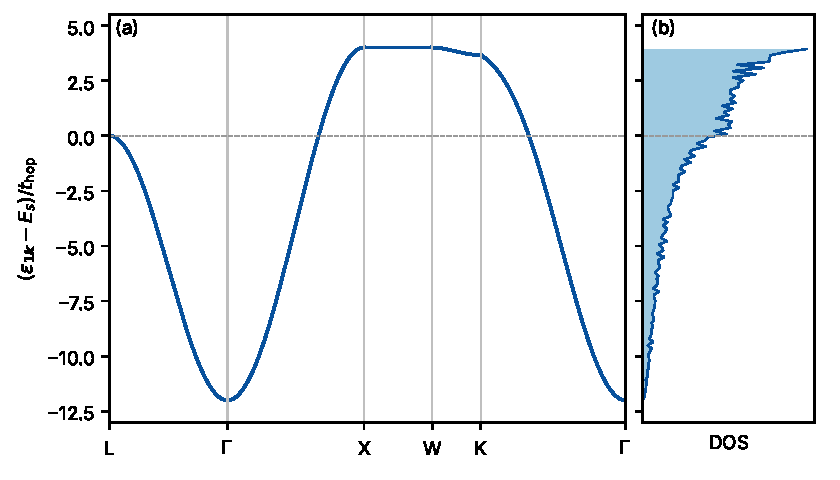
\includegraphics[width=0.75\linewidth]{figures/ch03/fig3_5.pdf}
  \caption{Tight-binding $s$ band of the face-centered cubic lattice, \cref{eq:3.2-fcc}: one orbital per site with on-site energy $E_s$, hopping $-t_{\mathrm{hop}}$ between the 12 nearest neighbors, no longer-range hopping, and the overlap between orbitals on different sites neglected. (a)~$(\varepsilon_{1\vect{k}} - E_s)/t_{\mathrm{hop}}$ along the path $\mathrm{L}$--$\mathrm{\Gamma}$--$\mathrm{X}$--$\mathrm{W}$--$\mathrm{K}$--$\mathrm{\Gamma}$, with $\mathrm{L} = (\tfrac12,\tfrac12,\tfrac12)$, $\mathrm{X} = (1,0,0)$, $\mathrm{W} = (1,\tfrac12,0)$ and $\mathrm{K} = (\tfrac34,\tfrac34,0)$ in units of $2\pi/a$. The band runs from $-12t_{\mathrm{hop}}$ at $\mathrm{\Gamma}$ to $+4t_{\mathrm{hop}}$, which it reaches at $\mathrm{X}$ and keeps along the line $\mathrm{X}$--$\mathrm{W}$; its value at $\mathrm{L}$ is $0$ and at $\mathrm{K}$ $3.66\,t_{\mathrm{hop}}$. (b)~Density of states, in arbitrary units, from a uniform grid of $160^3$ crystal momenta. Its peak at the top of the band comes from the flat line $\mathrm{X}$--$\mathrm{W}$.}
  \label{fig:3-tb}
\end{figure}

Silicon needs more than one orbital per atom, and the reason is chemical. A silicon atom has its $3s$ level several electronvolts below its $3p$ level, and in the crystal it uses both: it forms four bonds to the four neighbors of \cref{eq:3.1-basis}, at the corners of a tetrahedron. The orbitals that point along these bonds are the four $sp^3$ \emph{hybrids}
\begin{equation}
  \begin{aligned}
  h_1 &= \tfrac12(s + p_x + p_y + p_z), &\qquad h_2 &= \tfrac12(s + p_x - p_y - p_z), \\
  h_3 &= \tfrac12(s - p_x + p_y - p_z), &\qquad h_4 &= \tfrac12(s - p_x - p_y + p_z).
  \end{aligned}
  \label{eq:3.2-hybrids}
\end{equation}
These are orthonormal combinations of one $s$ and three $p$ orbitals on the same atom. Each is directed along one of the cube diagonals $(1,1,1)$, $(1,-1,-1)$, $(-1,1,-1)$ and $(-1,-1,1)$ that join an atom at $\vect{\tau}_1$ to its neighbors. Each hybrid has the on-site energy $(E_s + 3E_p)/4$, a quarter of the way from $E_p$ toward $E_s$. Forming the hybrids costs promotion energy, since an electron is moved from $s$ to $p$ character, and the bonds pay it back~\cite[Chap.~3]{harrison1980electronic}.

Two hybrids that point at each other across a bond, one on each atom, are coupled by a large matrix element, which we write $-V_{\mathrm{cov}}$ with $V_{\mathrm{cov}} > 0$ (Harrison's covalent energy). Treated alone, the pair is the two-orbital problem of \cref{sec:2.3}: a bonding combination $(h + h')/\sqrt2$ at $(E_s + 3E_p)/4 - V_{\mathrm{cov}}$ and an antibonding combination $(h - h')/\sqrt2$ at $(E_s + 3E_p)/4 + V_{\mathrm{cov}}$. A primitive cell holds two atoms and eight hybrids, which make four bonds, hence four bonding and four antibonding orbitals. Its eight valence electrons exactly fill the four bonding orbitals, two per bond, with opposite spins. The smaller couplings, between hybrids on the same atom and between neighboring bonds, then broaden the four bonding levels into four valence bands and the four antibonding levels into four conduction bands. The gap of silicon is the remnant of the bonding--antibonding splitting $2V_{\mathrm{cov}}$, reduced by these broadenings, and it survives because the splitting is larger than the bands are wide~\cite[Chap.~3]{harrison1980electronic}. This picture accounts for the count of \cref{sec:3.1}, four filled bands, without any reference to Bragg planes. It also explains where the valence charge sits: the bonding orbitals concentrate it between the atoms, in the bonds. This bond charge is not a sum of spherical atomic terms, and it gives the potential of silicon its (222) component; the (200) component stays zero by the glide symmetry (\cref{we:3-diamond}, \cref{app:C.17}). Germanium is bonded the same way, more weakly. In GaAs the two hybrids of a bond have different energies, the bond is partly ionic, and the gap is wider than the covalent splitting alone would give (\cref{sec:3.3}).

The nearly-free and the tight-binding pictures are two limits of the same problem, \cref{eq:3.2-Hk}, and both are approximations to it. Real valence states of silicon are well described by neither: they have the bonding character of the tight-binding picture, and the plane-wave content near the zone boundary that the nearly-free picture predicts. A first-principles calculation solves \cref{eq:3.2-Hk} in a plane-wave basis (\cref{sec:3.4,sec:3.5}), and Wannier functions (\cref{sec:3.6}) recover from it a set of localized orbitals in which the band structure has the tight-binding form of \cref{eq:3.2-LCAO}, with orthonormal orbitals and hopping integrals computed rather than guessed.

\subsection{The density vertex}

A dark-matter particle couples to the electrons through $n_e(\vect{q}) = \sum_j\ee^{\ii\vect{q}\cdot\vect{r}_j}$, and for independent electrons each transition moves one electron, with the single-particle matrix element $f_{i\to f}(\vect{q}) = \langle f|\ee^{\ii\vect{q}\cdot\vect{r}}|i\rangle$ of \cref{eq:2.2-ff} (\cref{eq:2.3-ph}). Between Bloch states this matrix element has a simple structure. Take $\psi_{n\vect{k}}$ as the initial state and $\psi_{m\vect{k}'}$ as the final one, with $\vect{k}$ and $\vect{k}'$ in the first zone. The momentum transfer lies on the same grid as the crystal momenta, since the dark-matter states are normalized in the same periodic box of volume $\Vol$ (\cref{sec:2.1}). With \cref{eq:3.2-bloch},
\begin{equation*}
  \langle\psi_{m\vect{k}'}|\ee^{\ii\vect{q}\cdot\vect{r}}|\psi_{n\vect{k}}\rangle
  = \frac1N\int_V\dd^3r\;\ee^{\ii(\vect{k}+\vect{q}-\vect{k}')\cdot\vect{r}}\,u^*_{m\vect{k}'}(\vect{r})\,u_{n\vect{k}}(\vect{r}) .
\end{equation*}
Split the crystal into cells, $\vect{r} = \vect{R} + \vect{x}$ with $\vect{x}$ in the cell at the origin. The product $u^*u$ is the same in every cell, and the phase factorizes into $\ee^{\ii(\vect{k}+\vect{q}-\vect{k}')\cdot\vect{R}}$ times its value at $\vect{x}$. The sum over cells is the lattice sum of \cref{eq:3.1-latticesum}, which equals $N$ if $\vect{k} + \vect{q} - \vect{k}'$ is a reciprocal-lattice vector $\vect{G}_{\mathrm{U}}$ and vanishes otherwise:
\begin{equation*}
  \langle\psi_{m\vect{k}'}|\ee^{\ii\vect{q}\cdot\vect{r}}|\psi_{n\vect{k}}\rangle
  = \delta_{\vect{k}',\,\vect{k}+\vect{q}-\vect{G}_{\mathrm{U}}}\int_\Omega\dd^3x\;\ee^{\ii\vect{G}_{\mathrm{U}}\cdot\vect{x}}\,u^*_{m\vect{k}'}(\vect{x})\,u_{n\vect{k}}(\vect{x}) .
\end{equation*}
This is the selection rule \cref{eq:3.1-selection}, now for one electron. The vector $\vect{G}_{\mathrm{U}}$ is the one that folds $\vect{k} + \vect{q}$ back into the first zone. It depends on $\vect{k}$ as well as on $\vect{q}$, and it is not in general the vector $\vect{G}_q$ nearest to $\vect{q}$ of \cref{eq:3.1-qsplit}. With the periodic gauge, $u_{m,\vect{k}+\vect{q}} = \ee^{-\ii\vect{G}_{\mathrm{U}}\cdot\vect{r}}u_{m\vect{k}'}$ by \cref{eq:A.5-periodic}, and the phase is absorbed into the final state:
\begin{keyresult}[Density vertex]
For $\vect{k}$ in the first zone and any $\vect{q}$, $\ee^{\ii\vect{q}\cdot\vect{r}}$ connects $\psi_{n\vect{k}}$ only to the states at crystal momentum $\vect{k} + \vect{q}$, folded back as $\vect{k}' = \vect{k} + \vect{q} - \vect{G}_{\mathrm{U}}$. The amplitude is the \emph{density vertex}
\begin{equation}
  \begin{aligned}
  \rho_{mn}(\vect{k},\vect{q}) &\equiv \langle\psi_{m,\vect{k}+\vect{q}}|\ee^{\ii\vect{q}\cdot\vect{r}}|\psi_{n\vect{k}}\rangle
  = \int_\Omega\dd^3r\;u^*_{m,\vect{k}+\vect{q}}(\vect{r})\,u_{n\vect{k}}(\vect{r}) \\
  &= \int_\Omega\dd^3r\;u^*_{m\vect{k}'}(\vect{r})\,\ee^{\ii\vect{G}_{\mathrm{U}}\cdot\vect{r}}\,u_{n\vect{k}}(\vect{r}),
  \end{aligned}
  \label{eq:3.2-rho}
\end{equation}
with $\rho_{nn}(\vect{k},0) = 1$. It is of order one and carries no factor of $N$. The Umklapp vector $\vect{G}_{\mathrm{U}}$ stays in the plane wave.
\end{keyresult}
The normalization $\rho_{nn}(\vect{k},0) = \int_\Omega|u_{n\vect{k}}|^2 = 1$ is that of \cref{eq:3.2-bloch}. The plane wave $\ee^{\ii\vect{G}_{\mathrm{U}}\cdot\vect{r}}$ in \cref{eq:3.2-rho} cannot be dropped. The overlap $\int_\Omega u^*_{m\vect{k}'}u_{n\vect{k}}$ without it is a different number, and it would make the vertex depend on $\vect{q}$ only through its reduced part. The crystal momentum changes by $\vect{q}$ modulo a reciprocal-lattice vector, but the wavefunction is probed by the whole $\vect{q}$, which is why \cref{sec:3.1} never folds it.

The plane-wave form of the vertex shows what happens to the momentum. We insert \cref{eq:3.2-pw} for both states in the cell integral of \cref{eq:3.2-rho} that carries $\ee^{\ii\vect{G}_{\mathrm{U}}\cdot\vect{r}}$. The cell integral of $\ee^{\ii(\vect{G}_{\mathrm{U}} + \vect{G} - \vect{G}')\cdot\vect{r}}$ is $\Omega\,\delta_{\vect{G}',\vect{G}+\vect{G}_{\mathrm{U}}}$, and
\begin{equation}
  \rho_{mn}(\vect{k},\vect{q}) = \sum_{\vect{G}}c^*_{m\vect{k}'}(\vect{G} + \vect{G}_{\mathrm{U}})\,c_{n\vect{k}}(\vect{G}),
  \qquad \vect{k}' = \vect{k} + \vect{q} - \vect{G}_{\mathrm{U}} .
  \label{eq:3.2-rhopw}
\end{equation}
Each plane-wave component of the initial state, with momentum $\vect{k} + \vect{G}$, is shifted by exactly $\vect{q}$ to $\vect{k}' + \vect{G} + \vect{G}_{\mathrm{U}}$, and the vertex is the overlap of the shifted state with the final one. Momentum is conserved component by component; the crystal only decides how the result is labeled. In the empty lattice, where each state is one plane wave, \cref{eq:3.2-rhopw} reduces to the momentum conservation of free electrons, and the distinction between normal and Umklapp processes is a matter of band labels. In a crystal the coefficients spread each state over many $\vect{G}$, and a large $|\vect{q}|$ picks out the overlap between the high-momentum tail of the initial state and the low-momentum part of the final one. In the notation of Ref.~\cite[Eqs.~(3.14)--(3.16)]{essig2016direct}, $c_{n\vect{k}}(\vect{G})$ is their $u_n(\vect{k} + \vect{G})$ and \cref{eq:3.2-rhopw} is their $f_{[n\vect{k},m\vect{k}',\vect{G}_{\mathrm{U}}]}$.

The vertices out of one state exhaust the probability. The periodic functions $u_{m,\vect{k}+\vect{q}}$, $m = 1, 2, \dots$, are the eigenfunctions of the Hermitian operator $H_{\vect{k}+\vect{q}}$ on one cell and form a complete orthonormal set there. Expanding $u_{n\vect{k}}$ in them and using its normalization,
\begin{equation}
  \sum_m|\rho_{mn}(\vect{k},\vect{q})|^2 = \sum_m\Bigl|\int_\Omega u^*_{m,\vect{k}+\vect{q}}\,u_{n\vect{k}}\Bigr|^2 = \int_\Omega|u_{n\vect{k}}|^2 = 1
  \label{eq:3.2-closure}
\end{equation}
for every $\vect{q}$. This is the closure relation of \cref{eq:2.2-closure} for a Bloch electron: a momentum transfer redistributes the electron over the bands at $\vect{k} + \vect{q}$ without changing its total weight. At small $q$ the weight stays in band $n$; at $q$ beyond a few reciprocal-lattice vectors it spreads over many high bands, and the transitions that a detector sees, into the conduction bands just above the gap, receive the fraction that \cref{we:3-vertex} illustrates.

In second quantization, \cref{eq:2.3-nq} in the Bloch basis becomes
\begin{equation}
  n_e(\vect{q}) = \sum_{s}\sum_{\vect{k}\in\mathrm{BZ}}\sum_{mn}\rho_{mn}(\vect{k},\vect{q})\,c^\dagger_{m,\vect{k}+\vect{q},s}\,c_{n\vect{k}s},
  \label{eq:3.2-ne}
\end{equation}
with $c_{m,\vect{k}+\vect{q},s} = c_{m\vect{k}'s}$ in the periodic gauge. The particle--hole matrix element of \cref{eq:2.3-ph} that takes an electron from a valence state $v\vect{k}$ to a conduction state $c\vect{k}'$ is $\rho_{cv}(\vect{k},\vect{q})$, and the independent-electron transition sum of \cref{eq:2.5-indep} becomes a sum of $|\rho_{cv}(\vect{k},\vect{q})|^2$ over $\vect{k}$, the valence and conduction bands, and spin. That sum, weighted by energy conservation, is the crystal form factor of Ref.~\cite[Eq.~(3.17)]{essig2016direct}, which \cref{sec:10.1} derives in the book's normalization. The counting of \cref{app:A.3} explains why no factor of $N$ appears in \cref{eq:3.2-rho}: one sum over $\vect{k}$ supplies a factor $N$, and the prefactor $2\pi/\Vol$ of the structure factor turns it into the intensive $2\pi/\Omega$.

\subsection{Velocity matrix elements}

Light of energy $\omega$ has the momentum $q = \omega$, a few electronvolts for visible and ultraviolet photons, and $10^{-3}$ of the zone size. Optical absorption probes the density vertex at small $q$, and there it is controlled by a second matrix element, that of the velocity. The momentum and velocity matrix elements between Bloch states at the same $\vect{k}$ are
\begin{equation}
  \begin{gathered}
  \vect{p}_{mn}(\vect{k}) = \langle\psi_{m\vect{k}}|\op{\vect{p}}|\psi_{n\vect{k}}\rangle = \int_\Omega\dd^3r\;u^*_{m\vect{k}}\,(\op{\vect{p}} + \vect{k})\,u_{n\vect{k}}, \\
  \vect{v}_{mn}(\vect{k}) = \langle\psi_{m\vect{k}}|\vect{v}|\psi_{n\vect{k}}\rangle, \qquad
  \vect{v} = \ii[H_{\mathrm{e}},\vect{r}] .
  \end{gathered}
  \label{eq:3.2-pv}
\end{equation}
The velocity operator is the time derivative of the position in the Heisenberg picture. For the local potential of \cref{eq:3.2-He}, $U(\vect{r})$ commutes with $\vect{r}$ and $\vect{v} = \op{\vect{p}}/m_e$, so that $\vect{v}_{mn} = \vect{p}_{mn}/m_e$. In plane waves, $\vect{p}_{mn}(\vect{k}) = \sum_{\vect{G}}c^*_{m\vect{k}}(\vect{G})(\vect{k} + \vect{G})c_{n\vect{k}}(\vect{G})$. The matrix elements of $\vect{r}$ itself between extended states are not defined as integrals over the crystal, but for $m \ne n$ the commutator gives them a meaning. Taking $\langle\psi_{m\vect{k}}|\cdot|\psi_{n\vect{k}}\rangle$ of $\vect{v} = \ii[H_{\mathrm{e}},\vect{r}]$,
\begin{equation}
  \langle\psi_{m\vect{k}}|\vect{r}|\psi_{n\vect{k}}\rangle = \frac{-\ii\,\vect{v}_{mn}(\vect{k})}{\varepsilon_{m\vect{k}} - \varepsilon_{n\vect{k}}}, \qquad m \ne n ,
  \label{eq:3.2-r}
\end{equation}
which is the form in which interband position matrix elements enter first-principles codes (\cref{app:E.4}).

The dependence of these matrix elements on $\vect{k}$ is easiest to handle through the operator $H_{\vect{k}}$ of \cref{eq:3.2-Hk}. Differentiating its definition, $\nabla_{\vect{k}}(\ee^{-\ii\vect{k}\cdot\vect{r}}H_{\mathrm{e}}\ee^{\ii\vect{k}\cdot\vect{r}}) = \ee^{-\ii\vect{k}\cdot\vect{r}}(-\ii\vect{r}H_{\mathrm{e}} + \ii H_{\mathrm{e}}\vect{r})\,\ee^{\ii\vect{k}\cdot\vect{r}}$, so
\begin{equation}
  \nabla_{\vect{k}}H_{\vect{k}} = \ee^{-\ii\vect{k}\cdot\vect{r}}\,\vect{v}\,\ee^{\ii\vect{k}\cdot\vect{r}}, \qquad
  \vect{v}_{mn}(\vect{k}) = \int_\Omega\dd^3r\;u^*_{m\vect{k}}\,(\nabla_{\vect{k}}H_{\vect{k}})\,u_{n\vect{k}} .
  \label{eq:3.2-dHk}
\end{equation}
For the local potential, $\nabla_{\vect{k}}H_{\vect{k}} = (\op{\vect{p}} + \vect{k})/m_e$; the identity holds for any Hamiltonian, nonlocal ones included. The group velocity and the $\vect{k}\cdot\vect{p}$ relation both follow by differentiating $H_{\vect{k}}u_{n\vect{k}} = \varepsilon_{n\vect{k}}u_{n\vect{k}}$ with respect to $\vect{k}$,
\begin{equation*}
  (\nabla_{\vect{k}}H_{\vect{k}})\,u_{n\vect{k}} + H_{\vect{k}}\nabla_{\vect{k}}u_{n\vect{k}} = (\nabla_{\vect{k}}\varepsilon_{n\vect{k}})\,u_{n\vect{k}} + \varepsilon_{n\vect{k}}\nabla_{\vect{k}}u_{n\vect{k}},
\end{equation*}
and projecting onto $u_{m\vect{k}}$. For $m = n$ the terms with $\nabla_{\vect{k}}u_{n\vect{k}}$ cancel, because $\langle u_{n\vect{k}}|H_{\vect{k}} = \varepsilon_{n\vect{k}}\langle u_{n\vect{k}}|$, and normalization leaves
\begin{keyresult}[Group velocity]
\begin{equation}
  \vect{v}^{\mathrm{g}}_n(\vect{k}) \equiv \nabla_{\vect{k}}\varepsilon_{n\vect{k}} = \vect{v}_{nn}(\vect{k}) .
  \label{eq:3.2-vg}
\end{equation}
The slope of a band is the expectation value of the velocity in the Bloch state.
\end{keyresult}
This is the Hellmann--Feynman theorem for the parameter $\vect{k}$. A wave packet built from states of band $n$ near $\vect{k}$ moves with $\vect{v}^{\mathrm{g}}_n$, the \emph{group velocity}~\cite[Chap.~8 and App.~E]{ashcroft1976solid}. For free electrons it is $\vect{k}/m_e$. On a Bragg plane its component along $\vect{G}$ vanishes, as the standing waves of the nearly-free picture require, and in the tight-binding band \cref{eq:3.2-fcc} it vanishes at $\mathrm{\Gamma}$, $\mathrm{X}$ and $\mathrm{L}$ and is at most of order $t_{\mathrm{hop}}a$. For $m \ne n$, and $\varepsilon_{m\vect{k}} \ne \varepsilon_{n\vect{k}}$, the projection gives instead
\begin{equation}
  \langle u_{m\vect{k}}|\nabla_{\vect{k}}u_{n\vect{k}}\rangle = \frac{\vect{v}_{mn}(\vect{k})}{\varepsilon_{n\vect{k}} - \varepsilon_{m\vect{k}}} ,
  \label{eq:3.2-dudk}
\end{equation}
the first-order change of $u_{n\vect{k}}$ along band $m$ when $\vect{k}$ moves; this is $\vect{k}\cdot\vect{p}$ perturbation theory~\cite[Chap.~2]{yu2010fundamentals}.

The optical limit of the vertex is now one line. Expand the final state, $u_{m,\vect{k}+\vect{q}} = u_{m\vect{k}} + \vect{q}\cdot\nabla_{\vect{k}}u_{m\vect{k}} + O(q^2)$, in the overlap $\int_\Omega u^*_{m,\vect{k}+\vect{q}}u_{n\vect{k}}$ of \cref{eq:3.2-rho}. The zeroth-order term $\langle u_{m\vect{k}}|u_{n\vect{k}}\rangle$ vanishes for $m \ne n$, and the first-order term is $\vect{q}\cdot\langle\nabla_{\vect{k}}u_{m\vect{k}}|u_{n\vect{k}}\rangle = \vect{q}\cdot\langle u_{n\vect{k}}|\nabla_{\vect{k}}u_{m\vect{k}}\rangle^*$. With \cref{eq:3.2-dudk}, with $n$ and $m$ exchanged, and the hermiticity of the velocity, $\vect{v}^*_{nm} = \vect{v}_{mn}$:
\begin{keyresult}[Optical limit of the density vertex]
\begin{equation}
  \rho_{mn}(\vect{k},\vect{q}) = \frac{\vect{q}\cdot\vect{v}_{mn}(\vect{k})}{\varepsilon_{m\vect{k}} - \varepsilon_{n\vect{k}}} + O(q^2), \qquad m \ne n .
  \label{eq:3.2-optical}
\end{equation}
An interband vertex vanishes linearly as $q \to 0$, with a slope set by the velocity matrix element and the transition energy. The intraband vertex tends to one, $\rho_{nn}(\vect{k},\vect{q}) = 1 + O(q)$.
\end{keyresult}
The same result follows from expanding the plane wave, $\ee^{\ii\vect{q}\cdot\vect{r}} \simeq 1 + \ii\vect{q}\cdot\vect{r}$, between states at the same $\vect{k}$, and using \cref{eq:3.2-r}, which is the route of \cref{eq:A.5-optical}. The expansion assumes that the phases of the states are chosen smoothly in $\vect{k}$ between $\vect{k}$ and $\vect{k} + \vect{q}$. Any other choice multiplies both sides of \cref{eq:3.2-optical} by phases (\cref{eq:A.5-gauge}), and leaves $|\rho_{mn}|^2$, which is what a first-order rate contains, unchanged. When band $m$ is degenerate at $\vect{k}$, only the sum of $|\rho_{mn}|^2$ over the degenerate partners is defined (\cref{app:A.5}).

The interband probability $|\rho_{mn}|^2$ therefore grows as $q^2$ at small $q$, like the dipole transition $1s \to 2p$ of hydrogen in \cref{sec:2.2}. The intraband vertex does not vanish, but in a full band it cannot act: the state at $\vect{k} + \vect{q}$ in the same band is occupied, and the term is Pauli blocked. Intraband transitions matter in metals, at the Fermi surface (\cref{sec:4.5}). For photons, \cref{eq:3.2-optical} is all that is needed. The absorption spectrum of a semiconductor is a sum over the squared components of $\vect{v}_{cv}(\vect{k})$ along the polarization of the light (\cref{sec:4.4,sec:4.6}). Absorbed bosonic dark matter, whose momentum is also far below the zone scale (\cref{sec:3.3}), is governed by the same matrix elements (\cref{sec:10.7}).

The expansion of $u_{m,\vect{k}+\vect{q}}$ is useful while its first-order term is small, and by \cref{eq:3.2-dudk} this requires
\begin{equation}
  q \ll \frac{|\varepsilon_{m\vect{k}} - \varepsilon_{n\vect{k}}|}{|\vect{v}_{mn}(\vect{k})|} .
  \label{eq:3.2-validity}
\end{equation}
For a photon, with $q = \omega \simeq |\varepsilon_{m\vect{k}} - \varepsilon_{n\vect{k}}|$, the condition reads $|\vect{v}_{mn}| \ll 1$, the speed of light, and it always holds. For dark matter that deposits the same energy, the momentum transfer is at least $\omega/v_{\mathrm{max}}$ (\cref{sec:1.3}), and the condition becomes $|\vect{v}_{mn}| \ll v_{\mathrm{max}} = 2.650\times10^{-3}$. Valence electrons, however, move with typical velocities $\sim\alpha$, and the Fermi velocity of silicon's valence density is $7.0\times10^{-3}$ (\cref{sec:2.5}). Parametrically, then, the momentum transfers at which dark matter can excite an electron across the gap lie at or beyond the edge of the optical limit. \Cref{eq:3.2-optical} is a check on a calculation of $\rho_{mn}$ at small $q$, and a scattering rate needs the full vertex of \cref{eq:3.2-rhopw}.

In practice, the band energies $\varepsilon_{n\vect{k}}$ and the periodic parts $u_{n\vect{k}}$ of a real material come from density-functional theory (\cref{sec:3.4}). A code solves \cref{eq:3.2-central} for the Kohn--Sham potential in a basis of plane waves up to a cutoff (\cref{sec:3.5}) and stores the coefficients $c_{n\vect{k}}(\vect{G})$ on a grid of crystal momenta. The vertex is then the sum \cref{eq:3.2-rhopw}, with the coefficients of the two states matched by the integer coordinates of their $\vect{G}$. For all $\vect{G}_{\mathrm{U}}$ at once it is a fast Fourier transform of the product $u^*_{m\vect{k}'}u_{n\vect{k}}$, and the momentum matrix element is the corresponding sum over $\vect{k} + \vect{G}$ (\cref{app:E.7}). The pseudopotentials of these codes are nonlocal, and then $\vect{v} \neq \op{\vect{p}}/m_e$: by \cref{eq:3.2-dHk}, $\vect{v}_{mn}$ acquires the derivative of the nonlocal potential with respect to $\vect{k}$, a correction that \cref{app:E.7} evaluates and that changes the computed absorption of diamond by \SIrange{15}{20}{\percent}~\cite[Fig.~1]{ismailbeigi2001coupling}.

\begin{workedexample}{The vertex between the two lowest nearly-free bands}\label{we:3-vertex}
Return to the one-dimensional crystal of \cref{we:3-gap1d}, and take the initial state at the left zone boundary, $k = -\pi/a = -G_1/2$, in the lowest band, with the final state in the second band. Near the boundary the two bands are made of the plane waves $\ee^{\ii kx}$ and $\ee^{\ii(k+G_1)x}$, and \cref{eq:3.2-twowave}, with $\vect{G} \to -G_1$, mixes them. Its lower eigenvector is $(c(0), c(G_1)) = (\cos\theta_k, \sin\theta_k)$ and its upper one $(-\sin\theta_k, \cos\theta_k)$, with $\tan2\theta_k = 2|U_{G_1}|/(\varepsilon^0_{k+G_1} - \varepsilon^0_k)$; for $U_{G_1} < 0$ both components of the lower state have the same sign. At the boundary the two free energies are equal and $\theta = \pi/4$.

\emph{Small $q$.} For $0 < q < G_1$, $k + q$ stays in the first zone, $\vect{G}_{\mathrm{U}} = 0$, and \cref{eq:3.2-rhopw} reads $\rho_{21}(k,q) = -\sin\theta_{k+q}\cos\theta_k + \cos\theta_{k+q}\sin\theta_k = \sin(\theta_k - \theta_{k+q})$. With $\varepsilon^0_{k+G_1} - \varepsilon^0_k = G_1(k + G_1/2)/m_e$, the angle falls from $\pi/4$ with the slope $\dd\theta/\dd k = -G_1/(4m_e|U_{G_1}|)$ at the boundary, and
\begin{equation*}
  |\rho_{21}(k,q)| \simeq \frac{qG_1}{4m_e|U_{G_1}|} = \frac{q}{\SI{448}{eV}} .
\end{equation*}
The optical limit agrees. In the two-wave model $|v_{21}| = G_1/2m_e = 2.23\times10^{-3}$, the velocity of a free electron at the zone boundary, and \cref{eq:3.2-optical} gives $q|v_{21}|/2|U_{G_1}|$, the same expression. The full calculation of \cref{fig:3-nfe}(b) has $|v_{21}| = 2.24\times10^{-3}$ and $\varepsilon_{2k} - \varepsilon_{1k} = \SI{0.998}{eV}$. At $q = \SI{10}{eV}$ the vertex is $0.0225$ in the full calculation and in the optical limit; at \SI{100}{eV} the two are 0.210 and 0.225. At $q = 2|U_{G_1}|/v_{\mathrm{max}} = \SI{377}{eV}$, the smallest momentum transfer with which dark matter can deposit the \SI{1}{eV} gap, the full vertex is 0.496 and the optical limit 0.849, too large by a factor of 1.7, and $|\rho_{21}|^2$ by a factor of 2.9. This $q$ is a reference scale, not an allowed event, since the vertex is evaluated at fixed $k$: at $q = \SI{377}{eV}$ the final state from this $k$ has moved up the second band, the transition costs \SI{1.6}{eV}, and depositing \SI{1.6}{eV} needs $q \ge \SI{0.61}{keV}$. The vertex saturates instead of growing: as $k + q$ moves away from the boundary, the final state becomes a single plane wave, and $|\rho_{21}|$ tends to $\sin(\pi/4) = 0.71$ in the two-wave model. The scale on which the linear law fails, $4m_e|U_{G_1}|/G_1 = \SI{448}{eV}$, is the $|\varepsilon_{2k} - \varepsilon_{1k}|/|v_{21}|$ of \cref{eq:3.2-validity}, and $|v_{21}| = 0.85\,v_{\mathrm{max}}$ puts the momentum transfers of dark matter right at it.

\emph{Umklapp.} Now take $q = G_1 = \SI{2.28}{keV}$. Then $k + q = +\pi/a$, which is folded back to $k' = -\pi/a$ with $\vect{G}_{\mathrm{U}} = G_1$: the final state has the same reduced crystal momentum as the initial one, and the transition energy is the same \SI{0.998}{eV} as at $q \to 0$. At the boundary the states are $(c(0), c(G_1)) = (1, 1)/\sqrt2$ in band 1 and $(-1, 1)/\sqrt2$ in band 2. In \cref{eq:3.2-rhopw} only the term $\vect{G} = 0$ survives in the two-wave model, $c^*_{2k'}(G_1)\,c_{1k}(0) = \tfrac12$, so $|\rho_{21}(k, G_1)| = \tfrac12$; the full calculation finds 0.501. The same pair of states, with the same transition energy, has the vertex 0.02 at $q = \SI{10}{eV}$ and 0.50 at $q = G_1$. The difference comes from $\vect{G}_{\mathrm{U}}$ in the plane wave: the momentum transfer $G_1$ moves the component $\ee^{\ii kx}$ of the initial state onto the component $\ee^{\ii(k'+G_1)x}$ of the final one, and these overlap at order one. In the two-wave model band 2 receives a quarter of the probability and band 1 keeps another quarter. The remaining half, from the component $\ee^{\ii(k+G_1)x}$ shifted to $\ee^{\ii(k+2G_1)x}$, goes into bands 3 and 4, whose energies at the boundary are near $(3G_1/2)^2/2m_e = \SI{11.5}{eV}$. The full calculation finds $|\rho_{m1}|^2 = 0.298$, 0.251, 0.226 and 0.225 for $m = 1$ to 4, and the closure relation \cref{eq:3.2-closure} holds to $10^{-10}$.
\end{workedexample}

A one-dimensional cosine potential has two parameters and silicon has many. The lessons carry over, however: interband vertices are suppressed as $q$ at small momentum transfer, they saturate on the scale where the states change across the zone, and an Umklapp vector in the plane wave can make them of order one. Where the band edges of silicon, germanium and GaAs lie, and how large the relevant velocities and gaps are, is the subject of \cref{sec:3.3}.
